\begin{minipage}[t]{180mm}
\fcolorbox{black}{white}{
\begin{minipage}[b]{30mm}
\includegraphics[width=0.5\linewidth]{unflogo.pdf}
\end{minipage}
\begin{minipage}[b]{100mm}
\Huge \textbf{UNF NEWZ} \\
\Large -- jyder er også hvirveldyr!
\end{minipage}
\begin{minipage}[b]{50mm}
\Large Søndag 15.07.2013 \\
\normalsize Redigeret i \LaTeX\ af \\ SOM, MGS, KUM, TAL, JAM
\end{minipage}
}
\end{minipage}



\begin{minipage}[b]{0.95\linewidth}
\begin{minipage}[t]{0.47\textwidth}
\vspace{3mm}
\section*{Koordinativ Resolution}

Paa Campens derom nedlagte allerunderdanigste Forestilling har det under den femtende i Ormemaaneden i det tohundredeseksogtredivte Aar behaget mig, Campens Koordinator af Gauss' Naade, Eulers Husholder og Galois' ydmyge Efterfølger, at afstaa al Eierskab af Husalfen i en begrænset Periode mellem Solopgang og Solnedgang denne femtende i Ormemaaneden i det tohundredeseksogtredivte Aar. Dette vil dog ingenlunde begrænse Husalfens Forpligtelser, hverken over for Campen eller over for dens Tjenestemænd. Under mit Eierskabs Fravær paalægges Ansvaret for Tilsynet over Husalfens Ve, Vel og Opførsel det til dette Formaal nedsatte Konsistorium, bestaaende af de Arrangører paa Campen hvis upaaklagelige Ry gør dem egnet til Hvervet. Exekutivt opretholdes den Gaussgivne orden af de dertil udpegede Campforstandere som udpeges fra de ikke-svenske af Landets enkeltsammenhængende Provinser og som for at dokumentere deres Representationsret forventes offentligt at anerkende deres Tilhørsforhold til Drøvtyggernes Loge, og samtidigt sværge deres afstandstagen fra Ordinatorens magtfuldkommenhed.

{\flushright\emph{Morten Grue Sørensen, Koordinator af Gauss' Naade }}

\section*{Campens forfatningsretlige status}
Det har i årevis været et omdiskuteret emne blandt lærde i sommerskoleforfatningsvidenskab, om campen som organisation skal anses som \emph{corporation sole} eller som \emph{corporation aggregate}. I lighed med forholdene, der gælder for den britiske krone, er førstnævnte den mest udbredte interpretation, og tydeligvis også den, der ligger til grund for ovenstående resolution. Samtidig bruger resolutionen dog campens flerpersonelle egenskab for at nedsætte et konsitorium, som overtager nogle af absolutens beføjelser i en begrænset periode. Dette minder om et typisk første skridt i vestlige monarkiers demokratiseringsproces. Da denne afståelse dog er begrænset til få timer, må vi nærmere anse resolutionen som et middel til at fatsholde den absolutte magt, på trods af en stærk opposition i arrangørkredsen, fremfor at anse dette for det første spæde skridt i en demokratiseringsproces. Absoluten er desuden kendt for tidligere at have afgivet magten til yngre kræfter, udelukkende for at erobre den tilbage med magt i efterfølgende år, og sende de demokratiske kræfter til strafophold i kolonierne, sammen med deres uskyldige, men ofte forræderiske familie. Sammenfattende må vi derfor observere, at campen forbliver monarkist, og dermed til stadighed er i et modsætningsforhold til de teknokratiske og oligarkiske forfatningsstrukturer vi observer på andre camps, dog primært i oversøiske territorier. Erfaringerne fra disse reformationsprocesser er dog brogede, og prægede af gennemgribende spritmisbrug.  Dette, og den omstændighed, at jeg er blevet truet med eksklusion og eksekution af Campmarskallatet, indebærer at jeg trygt anbefaler omretholdelsen af de Gaussgivne absolutisk-aksiomatiske magtstrukturer på campen.

{\flushright\emph{S.O.M., campforfatningsekspert}}

\end{minipage}
\hfill\begin{minipage}[t]{0.47\textwidth}

\vspace{1mm}
\tikzstyle{mybox} = [draw=white, fill=blue!20, very thick,
    rectangle, rounded corners, inner sep=10pt, inner ysep=20pt]
\tikzstyle{fancytitle} =[fill=red, text=white]

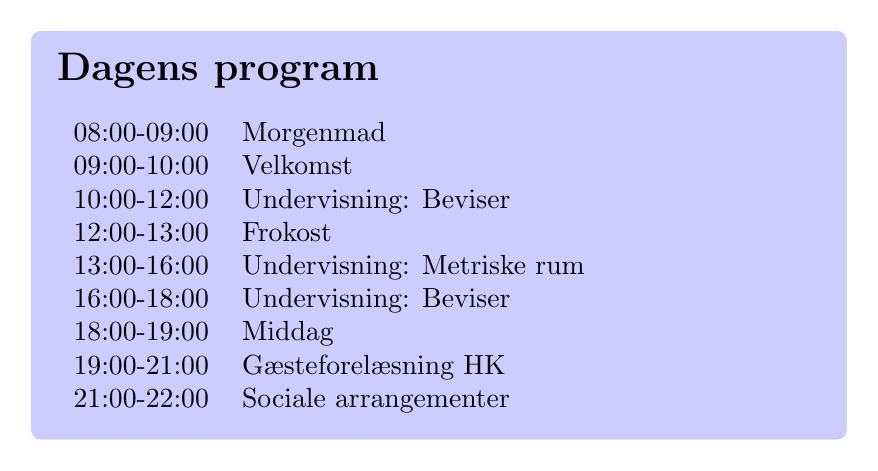
\begin{tikzpicture}
\node [mybox] (box){%
\begin{minipage}{0.80\textwidth}
\vspace{-4mm}\section*{Dagens program}
\begin{tabular}{ll}
08:00-09:00 & Morgenmad \\
09:00-10:00 & Velkomst \\
10:00-12:00 & Undervisning: Beviser \\
12:00-13:00 & Frokost \\
13:00-16:00 & Undervisning: Metriske rum \\
16:00-18:00 & Undervisning: Beviser \\
18:00-19:00 & Middag \\
19:00-21:00 & Gæsteforelæsning HK \\
21:00-22:00 & Sociale arrangementer
\end{tabular}
\vspace{-4mm}
\end{minipage}
};
\end{tikzpicture}%

\section*{Frygt ikke!}


\end{minipage}
\end{minipage}
